\vspace{-10pt}
\section{Evaluating Localization Ability of \gcam{}}
\subsection{Weakly-supervised Localization}\label{sec:localization}
In this section, we evaluate the localization capability of \gcam{} in the context of image classification.
The ImageNet localization challenge~\cite{imagenet_cvpr09} requires
approaches to provide bounding boxes in addition to classification labels.
Similar to classification, evaluation is performed for both the top-1 and top-5 predicted categories.

Given an image, we first obtain class predictions from our network and
then generate \gcam{} maps for each of the predicted classes and binarize them with a
threshold of 15\% of the max intensity.
This results in connected segments of pixels and we draw a bounding box around
the single largest segment.
Note that this is weakly-supervised localization -- the models were never exposed
to bounding box annotations during training.

We evaluate \gcam{} localization with off-the-shelf pretrained VGG-16~\cite{simonyan_arxiv14} \rpi{, AlexNet ~\cite{krizhevsky_nips12} and GoogleNet \cite{szegedy2016rethinking} 
(obtained from the Caffe~\cite{jia2014caffe} Zoo). }
Following ILSVRC-15 evaluation, we report both top-1 and top-5 localization errors
on the val set in \reftab{table:locres}.
\gcam{} localization errors are significantly better than those achieved by
c-MWP~\cite{zhang2016top} and Simonyan~\etal~\cite{simonyan_arxiv13}, which use grab-cut to
post-process image space gradients into heat maps.
\gcam{} for VGG-16 also achieves better top-1 localization error than CAM~\cite{zhou_cvpr16}, which requires a change
in the model architecture, necessitates re-training and thereby achieves worse classification errors (2.98\%
worse top-1), while \gcam{} does not compromise on classification performance.



\begin{table}[h!]
\vspace{-10pt}
\centering
    \resizebox{1.00\columnwidth}{!}{
        \begin{tabular}{l l l c c c c c c}
            & & \multicolumn{2}{c}{\textbf{Classification}} &~~~ & \multicolumn{2}{c}{\textbf{Localization}}\\
            \cmidrule{3-4}\cmidrule{6-7}
            & & \textbf{Top-$1$} & \textbf{Top-$5$} & & \textbf{Top-$1$} & \textbf{Top-$5$} \\
            \midrule
            \multirow{4}{*}{\rotatebox{90}{\tiny{\centering VGG-16}}} 

 &           Backprop~\cite{simonyan_arxiv13}   & $30.38$ & $10.89$ & & $61.12$ & $51.46$        \\
 &           c-MWP~\cite{zhang2016top}          & $30.38$ & $10.89$ & & $70.92$ & $63.04$        \\
&			\gcam{} (ours)                     & $30.38$ & $10.89$ & & $\mathbf{56.51}$ & $46.41$        \\
             \cmidrule{2-7}
&			CAM~\cite{zhou_cvpr16} & $33.40$ & $12.20$ & & $57.20$ & $\mathbf{45.14}$        \\
\midrule
\multirow{2}{*}{\rotatebox{90}{\tiny{\centering AlexNet}}} 
&           c-MWP~\cite{zhang2016top}          & $44.2$ & $20.8$ & & $92.6$ & $89.2$        \\
&			\gcam{} (ours)                     & $44.2$ & $20.8$ & & $68.3$ & $56.6$        \\
\midrule
\multirow{2}{*}{\rotatebox{90}{\tiny{\centering GoogleNet}}} 
&			\gcam{} (ours)                     & $31.9$ & $11.3$ & & $60.09$ & $49.34$        \\
&			CAM~\cite{zhou_cvpr16} 			   & $31.9$ & $11.3$ & & $60.09$ & $49.34$        \\
            \bottomrule
        \end{tabular}
    }
    \vspace{5pt}
    \caption{Classification and localization error \% on ILSVRC-15 val (lower is better) for VGG-16, AlexNet and GoogleNet. We see that \gcam{} achieves superior localization errors without compromising on classification performance.}
    \label{table:locres}
\end{table}

\vspace{-20pt}
\subsection{Weakly-supervised Segmentation}\label{sec:segmentation}

Semantic segmentation involves the task of assigning each pixel in the image an object class (or background class).
Being a challenging task, this requires expensive pixel-level annotation. 
The task of weakly-supervised segmentation involves segmenting objects with just image-level annotation, which can be obtained relatively cheaply from image classification datasets.
In recent work, Kolesnikov~\etal \cite{seed_eccv16} introduced a new loss function for training weakly-supervised image segmentation models.
Their loss function is based on three principles --
1) to seed with weak localization cues, encouraging segmentation network to match these cues,
2) to expand object seeds to regions of reasonable size based on information about which classes can occur in an image,
3) to constrain segmentations to object boundaries that alleviates the problem of imprecise boundaries already at training time.
They showed that their proposed loss function, consisting of the above three losses leads to better segmentation. 

However, their algorithm is sensitive to the choice of weak localization seed,
without which the network fails to localize objects correctly.
In their work, they used CAM maps from a VGG-16 based network which are used as object seeds for weakly localizing foreground classes.
We replaced the CAM maps with \gcam{} obtained from a standard VGG-16 network and obtain a Intersection over Union (IoU) score of 49.6 (compared to 44.6 obtained with CAM) on the PASCAL VOC 2012 segmentation task. \reffig{fig:segmentation_qual} shows some qualitative results.
% \rpi{More examples are available in \refsec{sec:sup_localization}.} %

\begin{figure}[htp]
\vspace{-17pt}
 \centering
 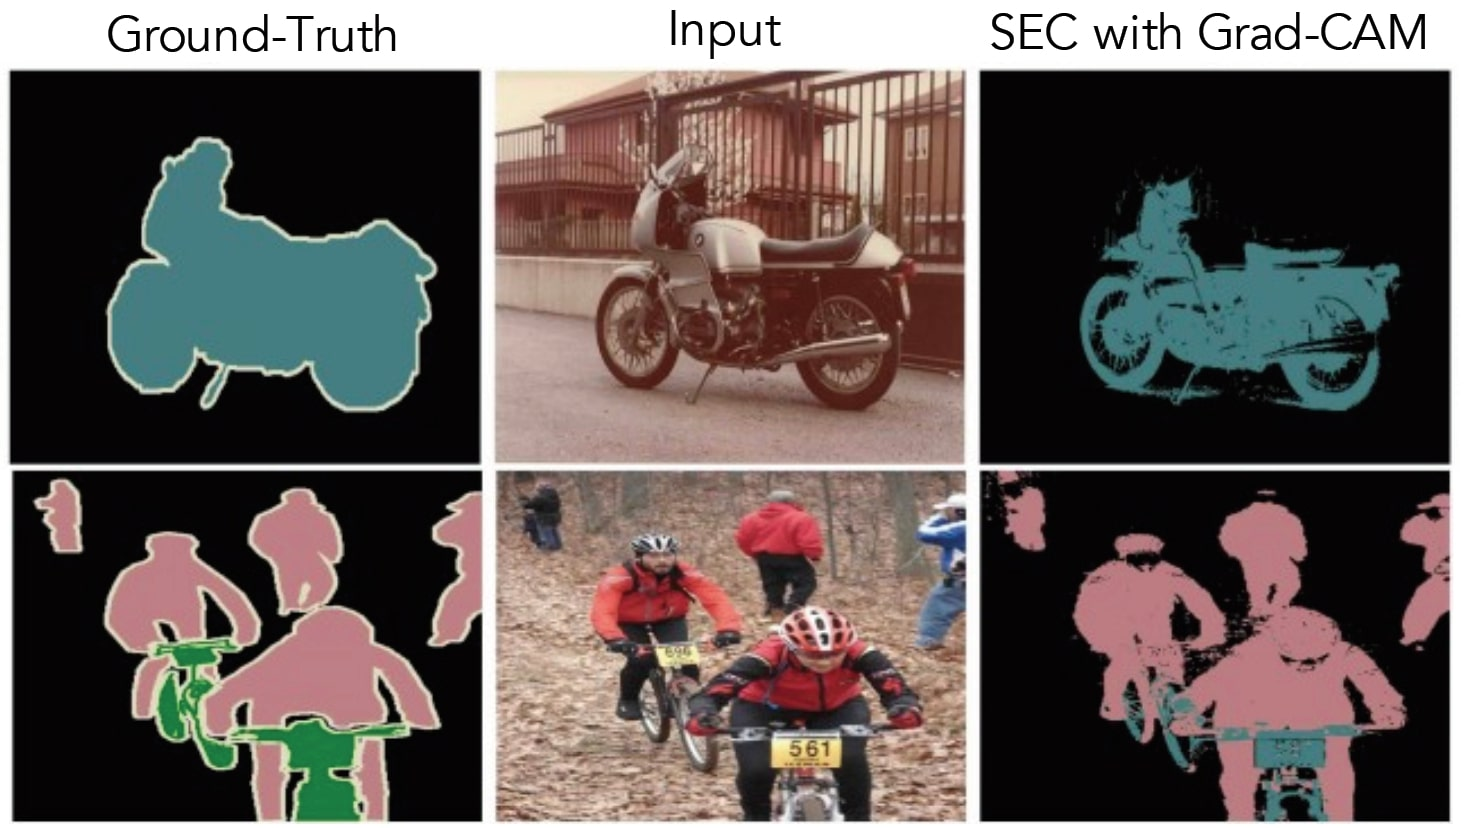
\includegraphics[width=1\linewidth]{figures/segmentation_qualitative.jpg}
 \caption{PASCAL VOC 2012 Segmentation results with \gcam{} as seed for SEC~\cite{seed_eccv16}.}
 \label{fig:segmentation_qual}
 \vspace{-10pt}
\end{figure}




\begin{figure*}[ht]
    \centering
   \begin{subfigure}[b]{0.25\textwidth}
       \centering
       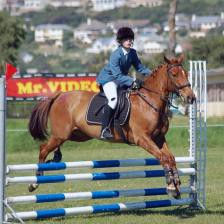
\includegraphics[width=0.55\linewidth]{figures/heval_1.jpg}
       \vspace{0.72in}
       \caption{\scriptsize{Raw input image. Note that this is not a part of the tasks (b) and (c)}}
		\label{fig:hs_clsdisc}
	\end{subfigure}
    \unskip\ \vrule\
   \hspace{0.05in}
    \begin{subfigure}[b]{0.25\textwidth}
        \centering
        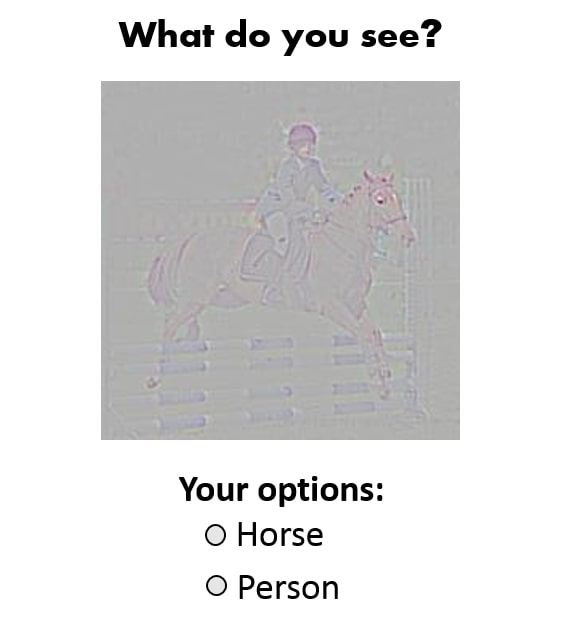
\includegraphics[width=0.90\linewidth]{figures/heval_2.jpg}
        \vspace{0.183in}
        \caption{\scriptsize{AMT interface for evaluating the class-discriminative property}}
		\label{fig:hs_clsdisc}
	\end{subfigure}
    \unskip\ \vrule\ \hspace{0.05in}
	\begin{subfigure}[b]{0.45\textwidth}
        \centering
        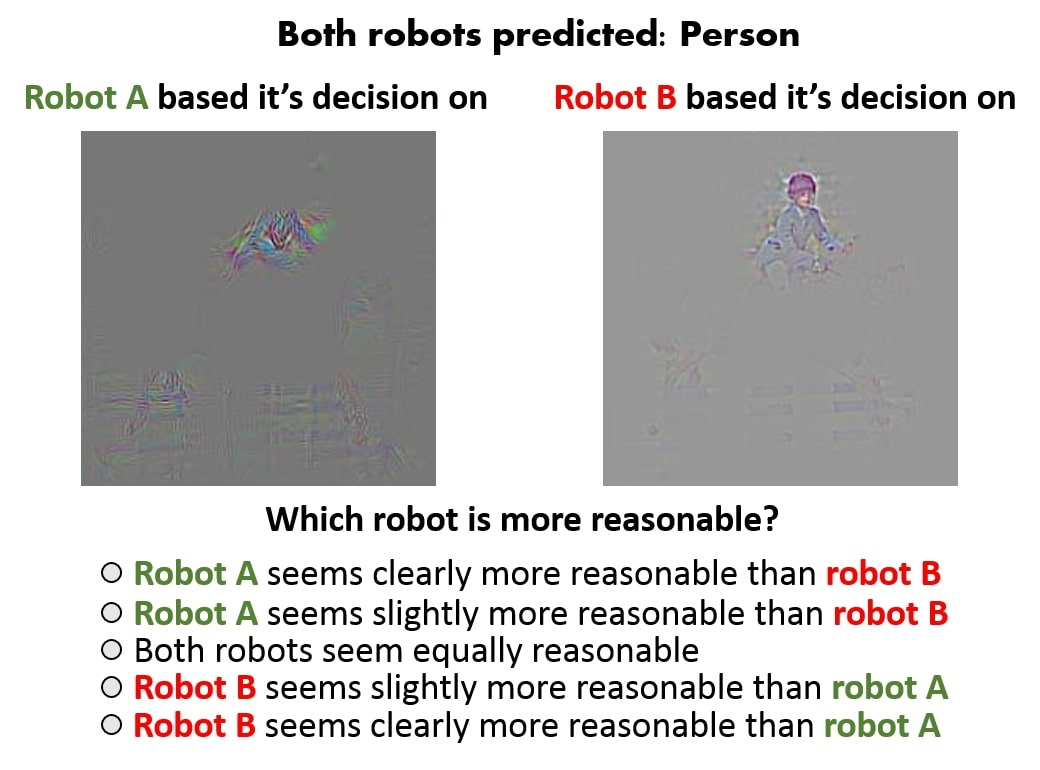
\includegraphics[width=0.95\linewidth]{figures/heval_3.jpg}
        \vspace{0.01in}
        \caption{\scriptsize{AMT interface for evaluating if our visualizations instill trust in an end user}}%
		\label{fig:hs_trust}
	\end{subfigure}
    \vspace{12pt}
	\caption{\rp{AMT interfaces for evaluating different visualizations for class discrimination (b) and trustworthiness (c). \cgb{} outperforms baseline approaches (Guided-backprop and \dec) showing that our visualizations are more class-discriminative and help humans place trust in a more accurate classifier.}}
\label{fig:human_studies}
\end{figure*}

\vspace{-15pt}
\subsection{Pointing Game}\label{sec:pointing_game}
\vspace{-2pt}

Zhang \etal~\cite{zhang2016top} introduced the Pointing Game experiment to evaluate the discriminativeness of
different visualization methods for localizing target objects in scenes.
Their evaluation protocol first cues each visualization technique with the ground-truth object label
and extracts the maximally activated point on the generated heatmap. 
It then evaluates if the point lies within one of the annotated instances of the target object category,
thereby counting it as a hit or a miss.

The localization accuracy is then calculated as \\$Acc = \frac{\#Hits}{\#Hits+\#Misses}$.
However, this evaluation only measures precision of the visualization technique.
We modify the protocol to also measure recall --
we compute localization maps for top-5 class predictions from the
CNN classifiers\footnote{We use GoogLeNet finetuned on COCO, as provided by ~\cite{zhang2016top}.}
and evaluate them using the pointing game setup with an additional option to
reject any of the top-5 predictions from the model if the maximally activated
point in the map is below a threshold,
\rp{\ie if the visualization correctly rejects the predictions which are absent
from the ground-truth categories, it gets that as a hit.}
We find that \gcam{} outperforms c-MWP~\cite{zhang2016top} by a significant
margin (70.58\% \vs 60.30\%).
Qualitative examples comparing c-MWP~\cite{zhang2016top} and \gcam{} on %
can be found in \secref{sec:sup_pointing}\footnote{
c-MWP~\cite{zhang2016top} highlights arbitrary regions for predicted but non-existent categories, unlike \gcam{} maps which typically do not.}.

